\documentclass[11pt,a4paper]{article}
\usepackage[T1]{fontenc}
\usepackage[utf8]{inputenc}
\usepackage{lmodern}
\usepackage{microtype}
\usepackage[margin=2.3cm]{geometry}
\usepackage{amsmath,amssymb,bm}
\usepackage{mathtools}
\usepackage{graphicx}
\usepackage{booktabs}
\usepackage{siunitx}
\usepackage[font=small,labelfont=bf]{caption}
\usepackage{xcolor}
\usepackage{enumitem}
\usepackage[section]{placeins}
\usepackage[hidelinks]{hyperref}
\usepackage[capitalise,noabbrev]{cleveref}
\setlist{itemsep=2pt,topsep=4pt}
\graphicspath{{../figs/}}
\sisetup{detect-all}
\setlength{\parskip}{3pt}

\DeclareMathOperator{\med}{med}
\DeclareMathOperator{\clip}{clip}
\newcommand{\vect}[1]{\bm{#1}}
\newcommand{\ind}{\mathbf{1}}
\newcommand{\Rvis}{R_{\mathrm{vis}}}
\newcommand{\Rall}{R_{\mathrm{all}}}
\newcommand{\etac}{\eta_{\mathrm{c}}}

\title{Locating Bragg Disks in CBED Patterns with a Disk--Ring Filter,\\ and Why Disk Overlap Makes It Hard}
\author{Diffraction project}
\date{November 2026}

\begin{document}
\maketitle

\begin{abstract}
\noindent
Bragg disks in a convergent-beam electron diffraction (CBED) pattern can be located without training by two steps:
a logarithmic intensity scale with a floor relative to the brightest pixel (\emph{true log}), and correlation with a
zero-mean template that compares a disk of the probe radius with a thin ring around it (\emph{disk--ring filter}). We
describe the method and evaluate it on 1\,875 simulated patterns (25 crystals, three probe angles, 25 thicknesses), scoring
every pattern separately. The single quantity that decides whether it works is the \emph{overlap ratio}
$\eta = 2r/s$, the disk diameter divided by the spacing between neighbouring reflections. While $\eta \lesssim 0.8$ the
filter's ring lies on background and almost every visible reflection is found, with a localisation error of
\SIrange{0.2}{0.3}{px}. Once the ring reaches the neighbouring disks, their intensity is subtracted from the response at the
true centre: the response there falls from a robust $z$-score of about 5 to near 0, the error grows to \SI{1}{px}, and
fewer than \SI{5}{\percent} of the lattice reflections are found when $\eta > 1.5$. A synthetic experiment that changes
only the disk size reproduces the collapse, and shows that interference between overlapping disks makes it worse. To keep
the disks separable, the probe semi-angle should not exceed $(s - \SI{3}{px})/(2\kappa)$, where
$\kappa \approx \SI{2.5}{px\per\milli\radian}$ is the disk radius per milliradian.
\end{abstract}

{\small\tableofcontents}

%══════════════════════════════════════════════════════════════════════════════
\section{Introduction}\label{sec:intro}
In CBED the incident beam is a cone of semi-angle $\alpha$, so every Bragg reflection appears as a disk rather than a spot.
The disk radius is set by the probe and grows with $\alpha$; the distance between disks is set by the crystal lattice and
does not. Locating the disks therefore becomes harder as $\alpha$ grows, because neighbouring disks approach, touch and
finally overlap (\cref{fig:geometry}).

This tutorial has two aims. The first is to describe a simple, training-free detector, true-log scaling followed by a
disk--ring matched filter (\cref{sec:method}), and to show how well it works when the disks are separate
(\cref{sec:results}). The second, and main, aim is to explain \emph{why} it fails when the disks overlap
(\cref{sec:overlap}). Everything is organised around one number, the overlap ratio
\begin{equation}
  \eta = \frac{2r}{s},
  \label{eq:eta}
\end{equation}
where $r$ is the disk radius and $s$ the distance between neighbouring reflections, both in pixels. Neighbouring disks touch
at $\eta = 1$. \Cref{sec:guide} turns the analysis into a rule for choosing $\alpha$.

\begin{figure}[!htbp]
  \centering
  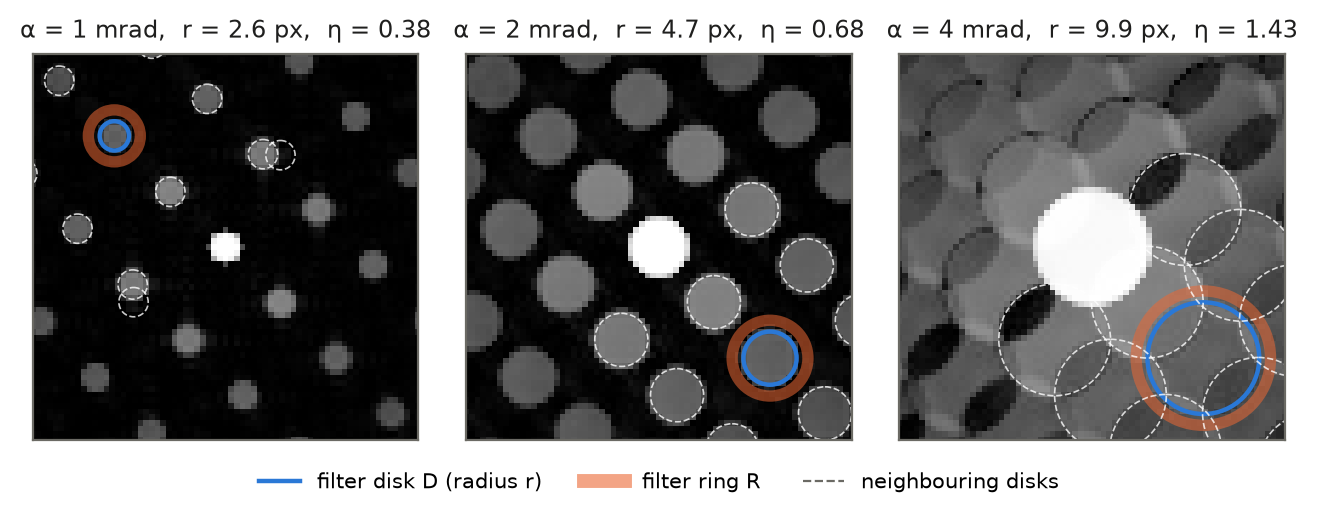
\includegraphics[width=\linewidth]{geometry.png}
  \caption{The same crystal (ZrSn$_3$, \SI{20}{\angstrom}) at three probe semi-angles. The lattice is unchanged; only the
  disks grow. The filter of \cref{sec:method} compares the mean inside a disk (blue) with the mean in a thin ring around it
  (orange). At 1 and \SI{2}{\milli\radian} the ring lies on dark background; at \SI{4}{\milli\radian}
  ($\eta = 1.43$) it lies on the neighbouring disks (dashed).}
  \label{fig:geometry}
\end{figure}

%══════════════════════════════════════════════════════════════════════════════
\section{Data and notation}\label{sec:data}
The patterns are multislice simulations (pyprismatic) of SiO$_2$ and 24 further crystals, each at probe semi-angles
$\alpha = 1$, 2 and \SI{4}{\milli\radian} and 25 thicknesses $t = 20, 40, \dots, \SI{500}{\angstrom}$: 1\,875 patterns in
total. Each simulation provides three arrays: $M$, the diffraction pattern; $V$, a map whose local maxima mark the
reciprocal-lattice points, used only for the ground truth; and $P$, the probe aperture, of which every disk is a shifted
copy. All processing uses the central $128 \times 128$ pixels of the $256 \times 256$ detector (\SI{0.02}{\per\angstrom}
per pixel). \Cref{tab:notation} lists the symbols used throughout.

\begin{table}[!htbp]
  \centering
  \caption{Notation.}
  \label{tab:notation}
  \small
  \begin{tabular}{ll}
    \toprule
    Symbol & Meaning \\
    \midrule
    $M$, $V$, $P$         & diffraction pattern, lattice-point map (ground truth only), probe aperture \\
    $T$                    & true-log image, \cref{eq:truelog} \\
    $\alpha$, $t$          & probe semi-angle (mrad), sample thickness (\si{\angstrom}) \\
    $r$, $\kappa$          & disk radius (px), from the probe, \cref{eq:probe}; $r \approx \kappa\alpha$ \\
    $s$                    & nearest-neighbour distance between lattice points (px) \\
    $\eta = 2r/s$          & overlap ratio; disks touch at $\eta = 1$ \\
    $D$, $R$; $g$, $w$     & filter disk and ring; gap and ring width ($g = \SI{1}{px}$, $w = \SI{2}{px}$) \\
    $K$, $S$, $z$          & kernel, filter response, robust $z$-score of the response \\
    $\Rvis$, $\Rall$       & per-image recall of visible reflections and of all lattice reflections, \cref{sec:eval} \\
    \bottomrule
  \end{tabular}
\end{table}

%══════════════════════════════════════════════════════════════════════════════
\section{Method: true log and disk--ring filter}\label{sec:method}

\subsection{True-log intensity scaling}
Disk intensities span several orders of magnitude: about $1$ for the direct beam, $10^{-2}$ for strong reflections and
$10^{-4}$ or less for weak ones (\cref{fig:pipeline}a). The common transform $\log(1+x)$ does not help here, because
$\log(1+x) \approx x$ for $x \ll 1$. Instead the logarithm is taken above a floor proportional to the brightest pixel.
With $x_{ij} = \max(M_{ij}, 0)$ and $m = \max_{ij} x_{ij}$,
\begin{equation}
  T_{ij} = \clip\!\left(
    \frac{\log_{10}(x_{ij} + \varepsilon m) - \log_{10}(\varepsilon m)}
         {\log_{10}(m + \varepsilon m) - \log_{10}(\varepsilon m)},\; 0,\; 1\right),
  \qquad \varepsilon = 10^{-4}.
  \label{eq:truelog}
\end{equation}
This maps the four decades between $\varepsilon m$ and $m$ onto $[0, 1]$, so weak and strong disks become comparable
(\cref{fig:pipeline}b). A larger $\varepsilon$ hides weak disks; a smaller one lifts the diffuse background above the floor.

\subsection{Disk radius from the probe}
The aperture image is close to binary. With $w(\vect u) = \ind[P(\vect u) > 0.5]$ the disk radius follows from its area,
\begin{equation}
  r = \sqrt{\frac{1}{\pi}\sum_{\vect u} w(\vect u)} ,
  \label{eq:probe}
\end{equation}
giving $r = 2.6$, $4.7$ and \SI{9.9}{px} at $\alpha = 1$, 2 and \SI{4}{\milli\radian}, that is $r \approx \kappa\alpha$ with
$\kappa \approx \SI{2.5}{px\per\milli\radian}$. The radius is the filter's only size parameter.

\subsection{Disk--ring matched filter}
A disk is a bright region of radius $r$ on a darker background. The filter compares a disk $D$ with a ring $R$ outside it,
separated by a gap $g$ so that the soft disk edge falls in neither:
\begin{equation}
  D = \{\vect u : \|\vect u\| \le r\}, \qquad
  R = \{\vect u : r + g < \|\vect u\| \le r + g + w\}.
  \label{eq:sets}
\end{equation}
The kernel is positive on $D$, negative on $R$, and sums to zero (\cref{fig:kernel}):
\begin{equation}
  K(\vect u) = \frac{\ind_D(\vect u)}{|D|} - \frac{\ind_R(\vect u)}{|R|} .
  \label{eq:kernel}
\end{equation}
The response at pixel $\vect p$ is therefore the mean of $T$ over the disk minus its mean over the ring:
\begin{equation}
  S(\vect p) = \sum_{\vect u} K(\vect u)\, T(\vect p + \vect u)
  = \underbrace{\frac{1}{|D|}\sum_{\vect u \in D} T(\vect p + \vect u)}_{\text{disk mean}}
  - \underbrace{\frac{1}{|R|}\sum_{\vect u \in R} T(\vect p + \vect u)}_{\text{ring mean}} .
  \label{eq:corr}
\end{equation}
$S$ is computed for all pixels at once by FFT convolution. The image is first extended by mirror reflection over the
kernel half-width, so that near the border the ring samples image-like values instead of zeros.

Two properties make this a matched filter for a disk. A uniform region gives $S = 0$, so smooth background is ignored;
and an isolated disk of height $h$ above its surroundings gives $S = h$ exactly at its centre, falling off-centre as part
of the disk enters the ring. Each disk therefore produces one maximum at its centre (\cref{fig:pipeline}c). Both properties
rely on one assumption: \emph{the ring lies on background}. \Cref{sec:overlap} is about what happens when it does not.

\begin{figure}[!htbp]
  \centering
  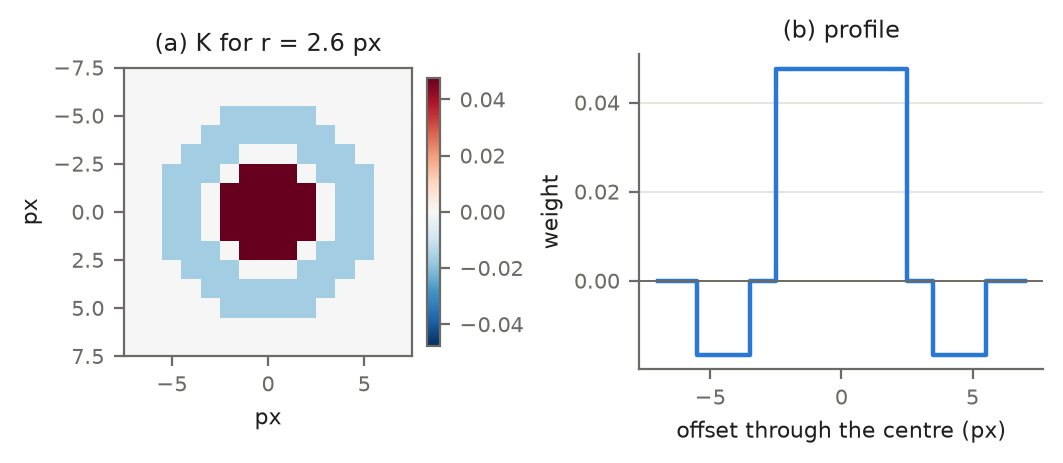
\includegraphics[width=0.8\linewidth]{kernel.png}
  \caption{Disk--ring kernel $K$ for $r = \SI{2.6}{px}$ (\SI{1}{\milli\radian}): (a) weights, (b) profile through the
  centre. Positive on the disk, negative on the ring, zero in the gap; the weights sum to zero.}
  \label{fig:kernel}
\end{figure}

\subsection{From response to disk centres}
The response is converted to a robust $z$-score, so that one threshold scale applies to all images:
\begin{equation}
  z(\vect p) = \frac{S(\vect p) - \med(S)}{1.4826\,\med\bigl(|S - \med(S)|\bigr)} .
  \label{eq:z}
\end{equation}
Candidate centres are the local maxima of $z$ in a $9 \times 9$ window (minimum separation $\rho = \SI{4}{px}$), refined to
sub-pixel precision by fitting a parabola through each maximum and its two neighbours along each axis. Each candidate keeps
its $z$ value as confidence; a threshold on $z$ selects the reported disks.

\begin{figure}[!htbp]
  \centering
  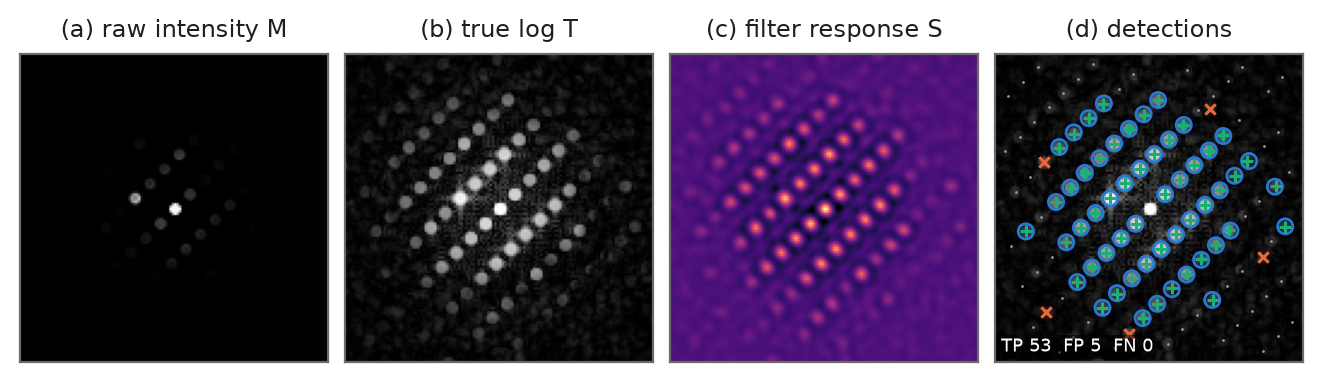
\includegraphics[width=\linewidth]{pipeline.png}
  \caption{The method on one pattern (SiO$_2$, \SI{1}{\milli\radian}, \SI{200}{\angstrom}): (a) raw intensity, dominated by
  the direct beam; (b) true log, \cref{eq:truelog}; (c) filter response, \cref{eq:corr}, one peak per disk; (d) detections
  at the threshold of this image (symbols as in \cref{fig:sio2}).}
  \label{fig:pipeline}
\end{figure}

%══════════════════════════════════════════════════════════════════════════════
\section{Evaluation}\label{sec:eval}

\paragraph{Lattice reflections.} The ground-truth centres are the local maxima of $V$ (in a $5 \times 5$ window, at least
\SI{5}{\percent} of the strongest reflection, direct beam excluded), refined by a $3 \times 3$ centroid. They do not depend
on $\alpha$ or $t$ and mark every reflection of the lattice, whether or not it is bright in $M$. The spacing $s$ is the
median distance from each lattice point to its nearest neighbour.

\paragraph{Visible reflections.} Many lattice reflections carry almost no intensity in $M$. A reflection is called
\emph{visible} if, in $M$, the mean over its disk is at least three times the mean over its ring (\cref{eq:sets}) and at least
$10^{-3}$ of the brightest disk.

\paragraph{Matching.} Detections are taken in order of decreasing $z$; one is correct if an unmatched reflection lies within
\SI{2}{px}. A detection on the direct beam is ignored.

\paragraph{Per-image recall.} Every image (one crystal, angle and thickness) is scored on its own; nothing is pooled across
thicknesses or angles. For each image the threshold is the lowest $z$ that keeps at most five false detections in that image,
and two recalls are reported:
\begin{equation}
  \Rvis = \frac{\text{visible reflections found}}{\text{visible reflections}}, \qquad
  \Rall = \frac{\text{lattice reflections found}}{\text{lattice reflections}} .
  \label{eq:recall}
\end{equation}
$\Rvis$ is computed only for images with at least three visible reflections. Summaries over crystals or thicknesses are
medians of these per-image values. The two recalls answer different questions: $\Rvis$ asks how well the detector finds
what is plainly there, $\Rall$ how much of the lattice it recovers. \Cref{sec:visible} shows why only $\Rall$ reveals the
effect of overlap.

%══════════════════════════════════════════════════════════════════════════════
\section{Results}\label{sec:results}

\subsection{Three example crystals}
\Cref{tab:examples} follows three crystals across the three probe angles. SiO$_2$ has a dense lattice
($s = \SI{8.6}{px}$); AlCo$_3$ and ZrSn$_3$ have wider spacings ($s \approx \SI{14}{px}$). Whenever $\eta < 0.8$, the filter
response at the true centres is high ($z = 2.4$--$5.8$), almost every visible reflection is found ($\Rvis = 0.94$--$1.00$)
and the correct detections lie within a quarter of a pixel at \SI{1}{\milli\radian}. When $\eta > 1$ the picture changes
in every column at once: the ring lies on neighbouring disks, the response at the centres drops to $1.2$ or less, few
reflections remain visible, and $\Rall$ falls to $0.02$--$0.30$. \Cref{fig:sio2} shows SiO$_2$ image by image.

\begin{table}[!htbp]
  \centering
  \caption{Three crystals at three probe angles. Values are medians over the 25 thicknesses of per-image quantities.
  Ring on neighbours: fraction of the filter ring lying inside other disks. $z$ at centres: filter response at the true
  lattice points, \cref{eq:z}. Error: distance of correct detections to the true centre (\SI{1}{px} $=$
  \SI{0.02}{\per\angstrom}). --: fewer than three visible reflections in (almost) every image.}
  \label{tab:examples}
  \small
  \begin{tabular}{l c c c c c c c c c}
    \toprule
    Crystal & $\alpha$ & $s$ & $\eta$ & Ring on & $z$ at & Visible & $\Rvis$ & $\Rall$ & Error \\
            & (mrad)   & (px) &       & neighb. & centres & per image & & & (px) \\
    \midrule
    SiO$_2$          & 1 & 8.6  & 0.60 & 0.00 & 4.13 & 63 & 0.97 & 0.65 & 0.20 \\
                     & 2 &      & 1.09 & 0.36 & 1.23 & 23 & 0.96 & 0.30 & 0.51 \\
                     & 4 &      & 2.29 & 1.00 & 0.26 & 0  & --   & 0.03 & --   \\
    \addlinespace
    AlCo$_3$         & 1 & 14.0 & 0.37 & 0.00 & 4.35 & 58 & 0.94 & 0.75 & 0.16 \\
                     & 2 &      & 0.67 & 0.00 & 2.40 & 43 & 0.94 & 0.54 & 0.49 \\
                     & 4 &      & 1.41 & 0.99 & 0.13 & 5  & 0.88 & 0.08 & 0.38 \\
    \addlinespace
    ZrSn$_3$         & 1 & 13.8 & 0.38 & 0.00 & 5.76 & 59 & 1.00 & 0.94 & 0.22 \\
                     & 2 &      & 0.68 & 0.00 & 2.46 & 50 & 0.97 & 0.72 & 0.42 \\
                     & 4 &      & 1.43 & 1.00 & 0.25 & 0  & --   & 0.02 & --   \\
    \bottomrule
  \end{tabular}
\end{table}

\begin{figure}[p]
  \centering
  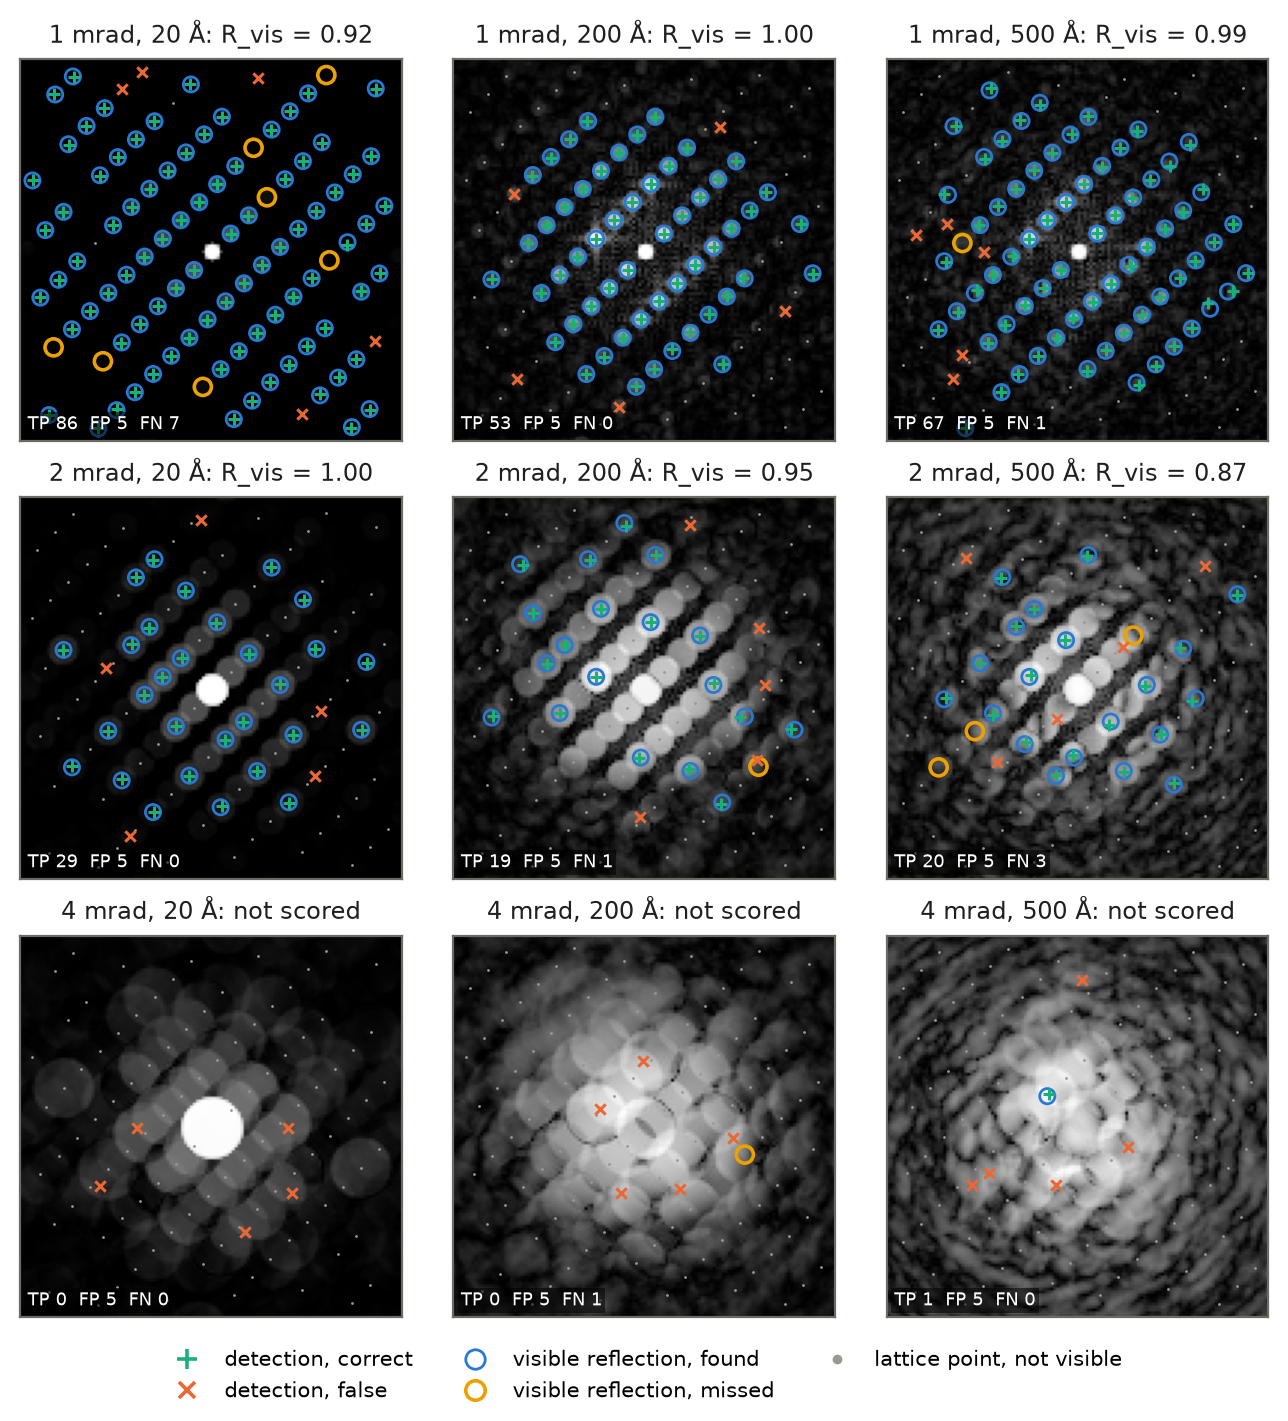
\includegraphics[width=\linewidth]{overlay_SiO2.png}
  \caption{SiO$_2$ at 1, 2, \SI{4}{\milli\radian} (rows; $\eta = 0.60$, $1.09$, $2.29$) and 20, 200, \SI{500}{\angstrom}
  (columns). Each image uses its own threshold (at most five false detections). Green $+$: correct detection; orange
  $\times$: false detection; blue circle: visible reflection found; yellow circle: visible reflection missed; grey dot:
  lattice point that is not visible. At \SI{4}{\milli\radian} no reflection is visible and the detections fall between
  lattice points.}
  \label{fig:sio2}
\end{figure}

\subsection{All 24 crystals}
\Cref{fig:crystals} shows $\Rvis$ for every image of the 24 crystals, with the crystals ordered by their spacing $s$ and the
overlap ratio printed next to each row. Two patterns stand out. Along each row, recall varies with thickness but rarely
collapses. Down the columns, the number of images that can be scored at all falls with $\eta$: at \SI{4}{\milli\radian},
where every crystal has $\eta > 1$, only 259 of 600 images contain three or more visible reflections, and the crystals with
the densest lattices have almost none. \Cref{tab:thick,fig:thick} give the thickness dependence: $\Rvis$ decreases slowly
with thickness at every angle, while $\Rall$ is set mainly by the angle (median $0.47$, $0.25$ and $0.04$ at
\SI{200}{\angstrom} for 1, 2 and \SI{4}{\milli\radian}).

\begin{figure}[!htbp]
  \centering
  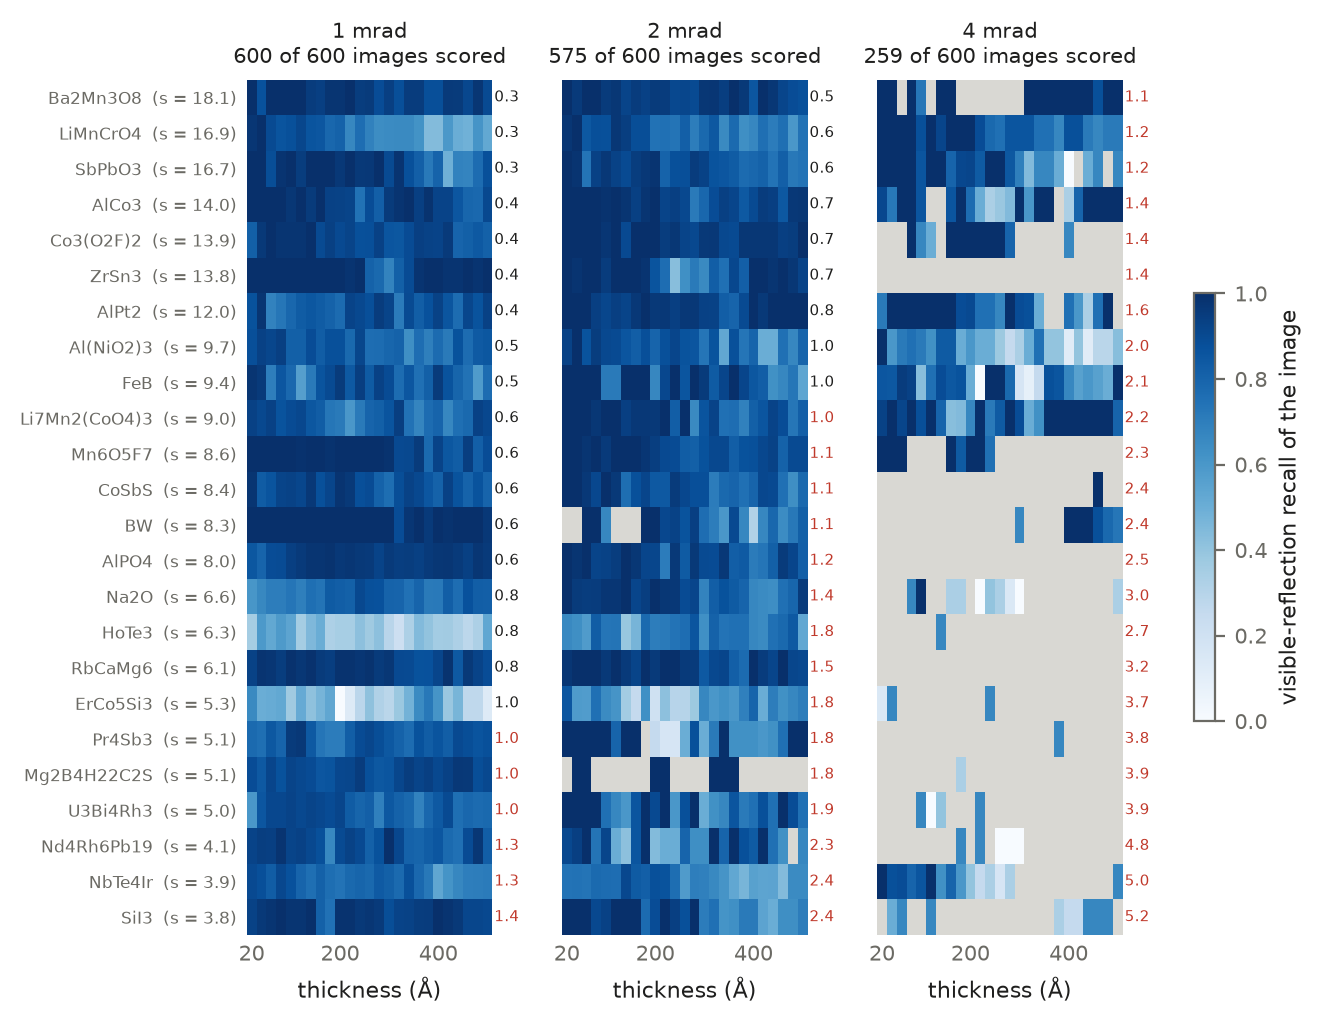
\includegraphics[width=\linewidth]{crystals24.png}
  \caption{$\Rvis$ of every image of the 24 crystals (rows) at 25 thicknesses (columns) and three probe angles (panels).
  Rows are sorted by spot spacing $s$, densest lattice at the bottom; the number to the right of each row is $\eta$ (red when
  $\eta \ge 1$). Grey: fewer than three visible reflections, not scored.}
  \label{fig:crystals}
\end{figure}

\begin{table}[!htbp]
  \centering
  \caption{24 crystals, per thickness: median over the crystals of the per-image recalls. $\Rvis$ uses images with at least
  three visible reflections (number of crystals in brackets); $\Rall$ uses all images. Median $\eta$: $0.62$, $1.13$ and
  $2.37$ at 1, 2 and \SI{4}{\milli\radian}.}
  \label{tab:thick}
  \small
  \begin{tabular}{c ccc ccc}
    \toprule
    & \multicolumn{3}{c}{$\Rvis$} & \multicolumn{3}{c}{$\Rall$} \\
    \cmidrule(lr){2-4}\cmidrule(lr){5-7}
    $t$ (\si{\angstrom}) & \SI{1}{\milli\radian} & \SI{2}{\milli\radian} & \SI{4}{\milli\radian}
                         & \SI{1}{\milli\radian} & \SI{2}{\milli\radian} & \SI{4}{\milli\radian} \\
    \midrule
    20  & 0.93 (24) & 1.00 (22) & 1.00 (11) & 0.74 & 0.33 & 0.08 \\
    100 & 0.93 (24) & 0.93 (23) & 0.86 (12) & 0.57 & 0.34 & 0.05 \\
    200 & 0.91 (24) & 0.91 (24) & 0.83 (10) & 0.47 & 0.25 & 0.04 \\
    300 & 0.86 (24) & 0.78 (23) & 0.68 (10) & 0.34 & 0.16 & 0.02 \\
    400 & 0.87 (24) & 0.80 (23) & 0.67 (11) & 0.26 & 0.13 & 0.02 \\
    500 & 0.88 (24) & 0.81 (23) & 0.72 (10) & 0.27 & 0.13 & 0.02 \\
    \bottomrule
  \end{tabular}
\end{table}

\begin{figure}[!htbp]
  \centering
  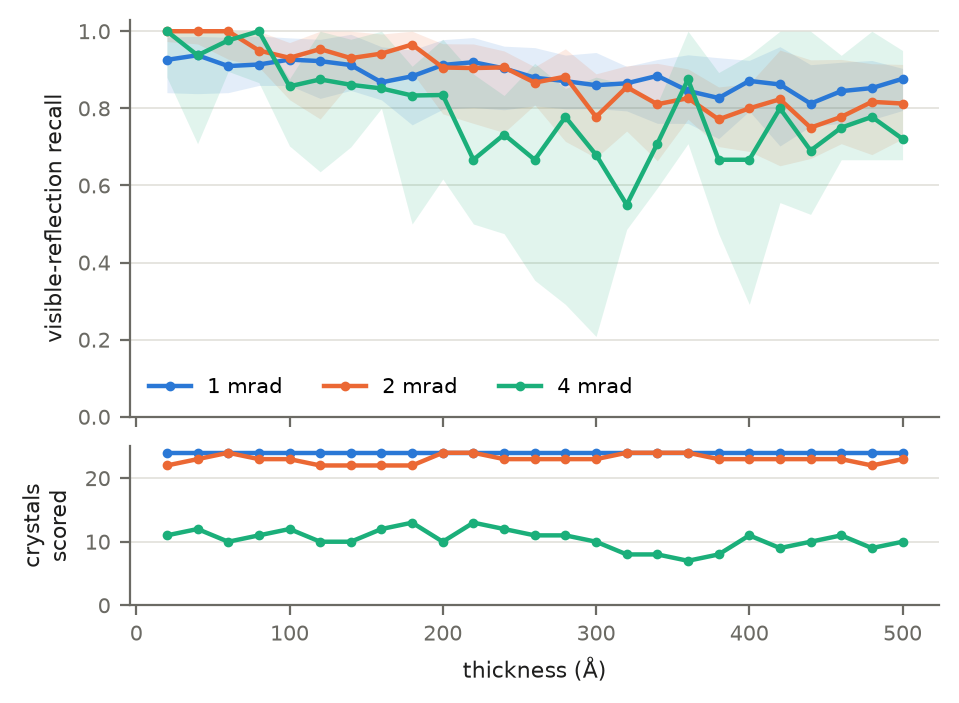
\includegraphics[width=0.72\linewidth]{thickness24.png}
  \caption{$\Rvis$ versus thickness for the 24 crystals: median (line) and middle \SI{50}{\percent} (band) over the crystals,
  and the number of crystals scored at each thickness (bottom).}
  \label{fig:thick}
\end{figure}

%══════════════════════════════════════════════════════════════════════════════
\section{Why disk overlap makes locating disks difficult}\label{sec:overlap}

\subsection{When does the ring reach the neighbours?}
The neighbouring disk begins at distance $s - r$ from a disk centre, and the filter ring ends at $r + g + w$
(\cref{eq:sets}). The ring stays on background as long as $r + g + w \le s - r$, that is
\begin{equation}
  \eta \le \etac = 1 - \frac{g + w}{s} .
  \label{eq:ringcond}
\end{equation}
For $s = \SI{14}{px}$, $\etac = 0.79$; for SiO$_2$ ($s = \SI{8.6}{px}$), $\etac = 0.65$. Disks touch at $\eta = 1$. Because
$r$ grows with $\alpha$ and $s$ is fixed, $\eta$ doubles each time $\alpha$ doubles: over the 24 crystals the median $\eta$ is
$0.62$, $1.13$ and $2.37$ at 1, 2 and \SI{4}{\milli\radian}, and 6, 15 and all 24 crystals have $\eta \ge 1$.

\subsection{What the filter measures under overlap}
For intuition, take linear intensities: a background $b$ plus disks of height $a_k$ centred at $\vect c_k$,
$I(\vect u) = b + \sum_k a_k\, \ind[\|\vect u - \vect c_k\| \le r]$. Inserting this into \cref{eq:corr} at the centre of
disk $0$ gives
\begin{equation}
  S(\vect c_0) = a_0 + \sum_{k \ne 0} a_k \bigl[\varphi_D(d_k) - \varphi_R(d_k)\bigr],
  \label{eq:response}
\end{equation}
where $d_k = \|\vect c_k - \vect c_0\|$ and $\varphi_D(d)$, $\varphi_R(d)$ are the fractions of the filter disk and of
the filter ring covered by a disk of radius $r$ at distance $d$. Three regimes follow:
\begin{enumerate}
  \item $d_k \ge 2r + g + w$ for all neighbours ($\eta \le \etac$): $\varphi_D = \varphi_R = 0$ and $S(\vect c_0) = a_0$.
        The response is the disk's own contrast, independent of its neighbours.
  \item $2r \le d_k < 2r + g + w$ ($\etac < \eta \le 1$): the disks do not yet touch, but $\varphi_R > 0$. Bright
        neighbours are \emph{subtracted}; a weak disk next to strong ones can get a negative response.
  \item $d_k < 2r$ ($\eta > 1$): the disks overlap and $\varphi_D > 0$ as well. Several neighbours cover the ring
        completely ($\varphi_R \to 1$), so the response at the centre becomes a difference of two sums of neighbour
        intensities with no particular sign. Meanwhile the lens-shaped regions where disks overlap form new bright
        patches of their own, which the filter can mistake for disks.
\end{enumerate}
The true-log transform is monotonic, so the same regimes apply to $T$, although the terms no longer add exactly.

\Cref{fig:overlap_real}a,b measures this on all 1\,875 images. The fraction of the ring lying on neighbouring disks is
zero up to $\eta \approx 0.8$ and reaches one beyond $\eta \approx 1.5$; of all the quantities measured it is the most
closely tied to $\eta$ (Spearman rank correlation $0.92$). The median response at the true centres falls with it, from
$z = 5.3$ for $\eta \le 0.5$ to $1.4$ at $0.8 < \eta \le 1$ and $0.03$ beyond $\eta = 2.5$ (\cref{tab:bins}): the true
centres stop standing out from the rest of the pattern.

\begin{figure}[!htbp]
  \centering
  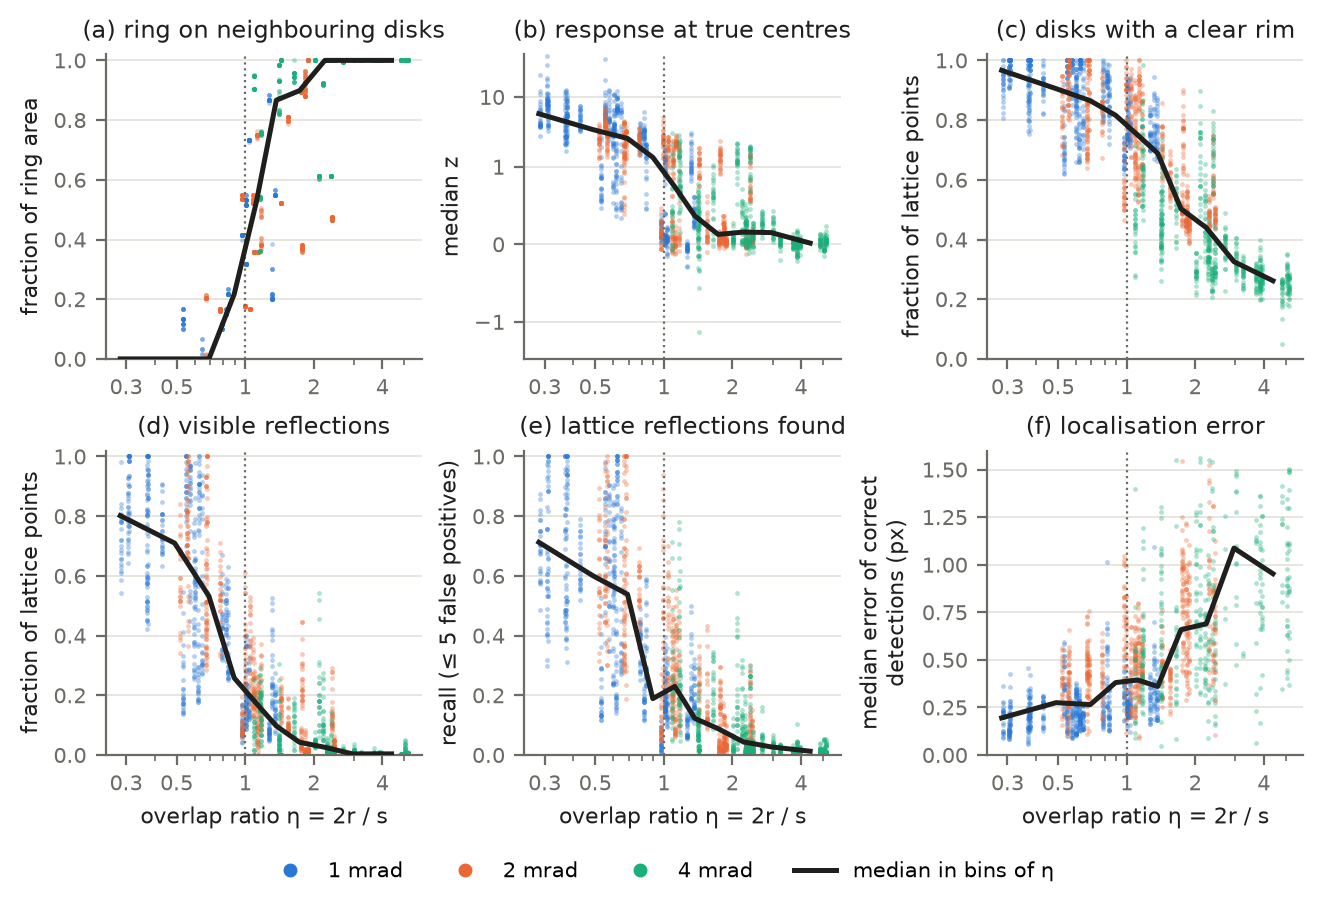
\includegraphics[width=\linewidth]{overlap_real.png}
  \caption{Every image of SiO$_2$ and the 24 crystals (dots, coloured by probe angle) versus its overlap ratio $\eta$; the
  black line is the median in bins of $\eta$; the dotted line marks $\eta = 1$. (a) Fraction of the filter ring lying on
  neighbouring disks. (b) Filter response at the true lattice points. (c) Fraction of lattice points whose disk still has a
  clear rim (intensity step of at least a factor $1.5$). (d) Fraction of lattice points that are visible. (e) $\Rall$.
  (f) Localisation error of correct detections.}
  \label{fig:overlap_real}
\end{figure}

\subsection{A controlled experiment}\label{sec:synthetic}
In real patterns several things change together with $\alpha$. To isolate overlap, we generated synthetic patterns in
which only the disk radius changes (\cref{fig:synthetic}): a square lattice with $s = \SI{14}{px}$ at a random rotation,
flat disks with a one-pixel soft edge, reflection intensities drawn log-uniformly between $10^{-3}$ and $10^{-1}$, a direct
beam of intensity 1 and a weak diffuse background. The radius runs from 2 to \SI{14}{px} ($\eta = 0.29$--$2.0$), with eight
patterns per radius. The disks are combined in two ways: \emph{incoherently}, $I = \sum_k I_k\,\ind_{D_k}$, and
\emph{coherently} with random phases, $I = \bigl|\sum_k \sqrt{I_k}\, e^{i\phi_k}\, \ind_{D_k}\bigr|^2$, which lets
overlapping disks interfere. All disks count as reflections to be found.

The result separates the two causes. In both models every disk is found as long as $\eta \le 0.86$, a little beyond
$\etac = 0.79$, while the response at the centres falls steadily from $z \approx 16$ to $3$ as the disks grow. At $\eta = 1$
recall drops to $0.81$, and beyond $\eta = 1.3$ the response at the centres is below $0.6$. With incoherent addition recall
then settles between $0.38$ and $0.54$: geometry alone, the ring on the neighbours, is enough to lose half of the disks.
With coherent addition it falls further, to $0.12$--$0.19$: interference makes some overlapping disks darker than their
surroundings, so even their own contrast $a_0$ in \cref{eq:response} changes sign.

\begin{figure}[!htbp]
  \centering
  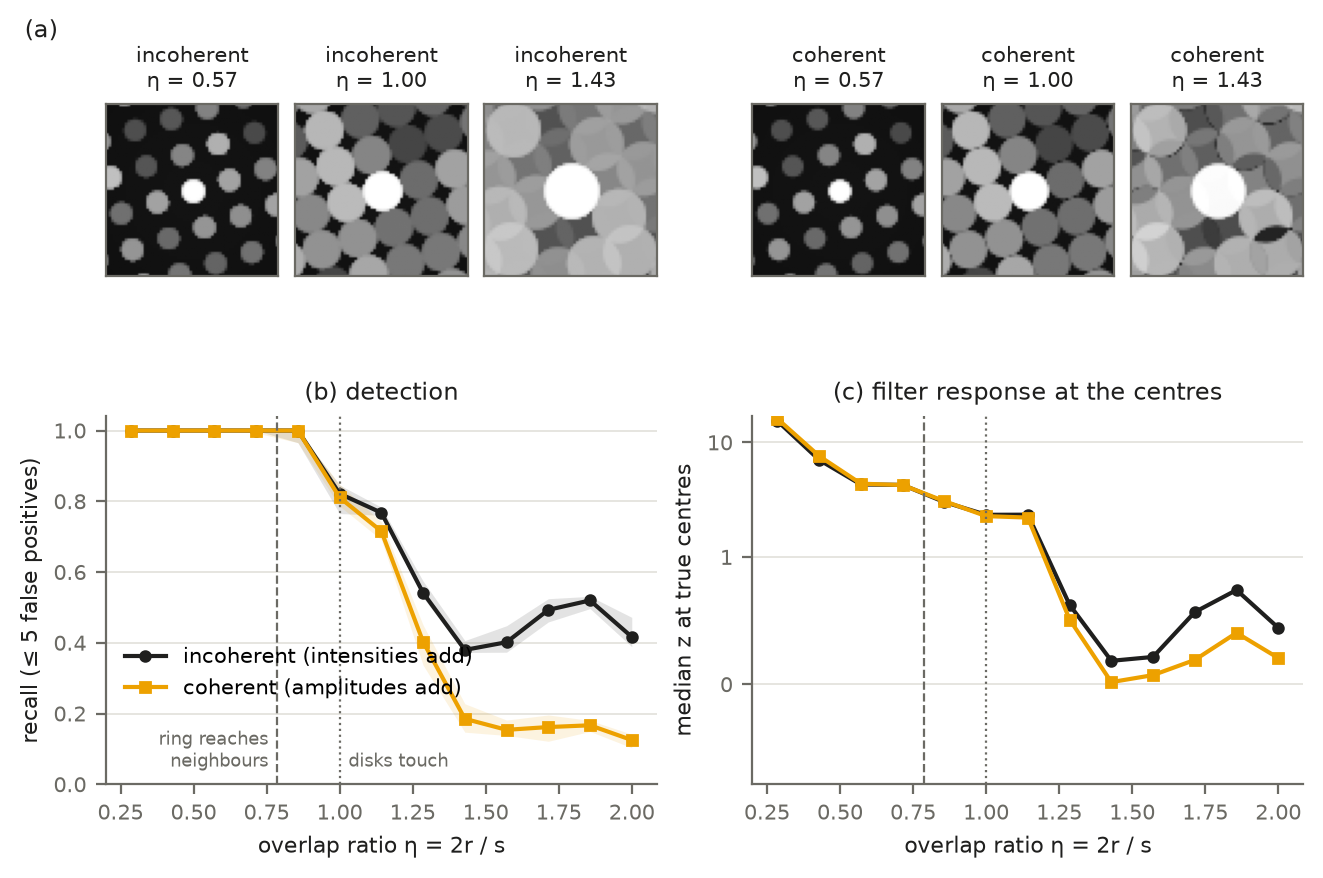
\includegraphics[width=\linewidth]{synthetic.png}
  \caption{Synthetic patterns in which only the disk radius changes ($s = \SI{14}{px}$). (a) True-log images at three
  overlap ratios, incoherent (left) and coherent (right) addition. (b) Recall at five false detections: median (line) and
  middle \SI{50}{\percent} (band) of eight patterns. (c) Median response at the true centres. Dashed line: $\etac = 0.79$,
  \cref{eq:ringcond}; dotted line: disks touch.}
  \label{fig:synthetic}
\end{figure}

\subsection{Disks lose their rim and their uniformity}
The disk model behind the filter, a flat disk with a sharp rim, also fails in the real patterns. \Cref{fig:overlap_real}c
counts the lattice points whose disk still shows a clear step in intensity across its rim. This fraction falls from
$0.95$ for $\eta \le 0.5$ to $0.48$ at $1.5 < \eta \le 2.5$ and $0.28$ beyond. Among the disks that do keep a clear rim,
the fraction that is \emph{darker} inside than outside rises from $0.02$ to $0.45$ over the same range (\cref{tab:bins}), as
in the coherent synthetic patterns. A dark disk has a negative response under \cref{eq:corr} and cannot be found by a
filter that looks for bright disks.

\subsection{Fewer visible reflections, and why \texorpdfstring{$\Rvis$}{R\_vis} hides the problem}\label{sec:visible}
The visibility test uses the same disk and ring as the filter: a reflection is visible if its disk is three times brighter
than its ring. Under overlap the ring contains neighbouring disks, so the test fails for the same reason the filter does.
The fraction of lattice points that are visible falls from $0.79$ for $\eta \le 0.5$ to $0.03$ at $1.5 < \eta \le 2.5$
(\cref{fig:overlap_real}d), and at \SI{4}{\milli\radian} the 24 crystals have a median of two visible reflections per
image.

As a consequence $\Rvis$ is almost independent of $\eta$ (Spearman $-0.15$): the reflections that are still visible are
precisely those whose surroundings remain dark, and the filter finds them. The loss appears instead in $\Rall$
(Spearman $-0.84$), which falls from $0.69$ for $\eta \le 0.5$ to $0.19$ at $0.8 < \eta \le 1.5$ and $0.02$ beyond
$\eta = 2.5$ (\cref{fig:overlap_real}e). Evaluating overlapped patterns with $\Rvis$ alone would therefore suggest that the
detector still works, when in fact most of the lattice is no longer recovered.

\subsection{Localisation becomes imprecise}
Even when a disk is found, overlap shifts its peak. Neighbours enter the ring on one side more than the other, which pulls
the maximum of $S$ away from the centre, and a large disk with internal structure gives a broad, uneven plateau rather than
a single sharp peak; with $r = \SI{9.9}{px}$ at \SI{4}{\milli\radian}, the peak window $\rho = \SI{4}{px}$ is also smaller
than the disk, so one disk can produce several maxima. The median error of correct detections grows from \SI{0.20}{px} for
$\eta \le 0.5$ to \SI{0.38}{px} around $\eta = 1$ and \SI{1.0}{px} beyond $\eta = 2.5$ (\cref{fig:overlap_real}f).

\begin{table}[!htbp]
  \centering
  \caption{All 1\,875 images (SiO$_2$ and 24 crystals) grouped by overlap ratio: medians of per-image quantities. Clear
  rim: lattice points with an intensity step of at least $\times 1.5$ across the rim; dark: fraction of those that are
  darker inside. Scored: fraction of images with at least three visible reflections.}
  \label{tab:bins}
  \small
  \begin{tabular}{l c c c c c c c c c}
    \toprule
    $\eta$ & Images & Ring on & $z$ at & Clear & Dark & Visible & Scored & $\Rall$ & Error \\
           &        & neighb. & centres & rim  &      & fraction &       &         & (px) \\
    \midrule
    $\le 0.5$     & 175 & 0.00 & 5.29 & 0.95 & 0.02 & 0.79 & 1.00 & 0.69 & 0.20 \\
    $0.5$--$0.8$  & 400 & 0.00 & 2.82 & 0.89 & 0.04 & 0.58 & 1.00 & 0.56 & 0.28 \\
    $0.8$--$1.0$  & 125 & 0.22 & 1.37 & 0.82 & 0.10 & 0.26 & 1.00 & 0.19 & 0.38 \\
    $1.0$--$1.5$  & 475 & 0.54 & 0.53 & 0.72 & 0.17 & 0.15 & 0.88 & 0.19 & 0.38 \\
    $1.5$--$2.5$  & 450 & 0.94 & 0.15 & 0.48 & 0.30 & 0.03 & 0.71 & 0.05 & 0.68 \\
    $> 2.5$       & 250 & 1.00 & 0.03 & 0.28 & 0.45 & 0.00 & 0.20 & 0.02 & 1.01 \\
    \bottomrule
  \end{tabular}
\end{table}

\subsection{Worst case: ZrSn\texorpdfstring{$_3$}{3} at 4 mrad}\label{sec:zrsn3}
ZrSn$_3$ shows all of these effects in one crystal (\cref{tab:examples,fig:zrsn3}). At 1 and \SI{2}{\milli\radian}
($\eta = 0.38$ and $0.68$, both below $\etac = 0.78$) it is one of the easiest crystals: $\Rvis = 1.00$ and $0.97$,
$\Rall = 0.94$ and $0.72$. At \SI{4}{\milli\radian} the same lattice gives $\eta = 1.43$. The ring lies entirely on
neighbouring disks, the response at the true centres falls from $5.8$ to $0.25$, only half of the lattice points keep a
clear rim, and in 24 of the 25 images no reflection is visible. The detector finds \SI{2}{\percent} of the lattice
reflections; its strongest responses lie on the direct beam and on the lens-shaped overlap regions.

\begin{figure}[p]
  \centering
  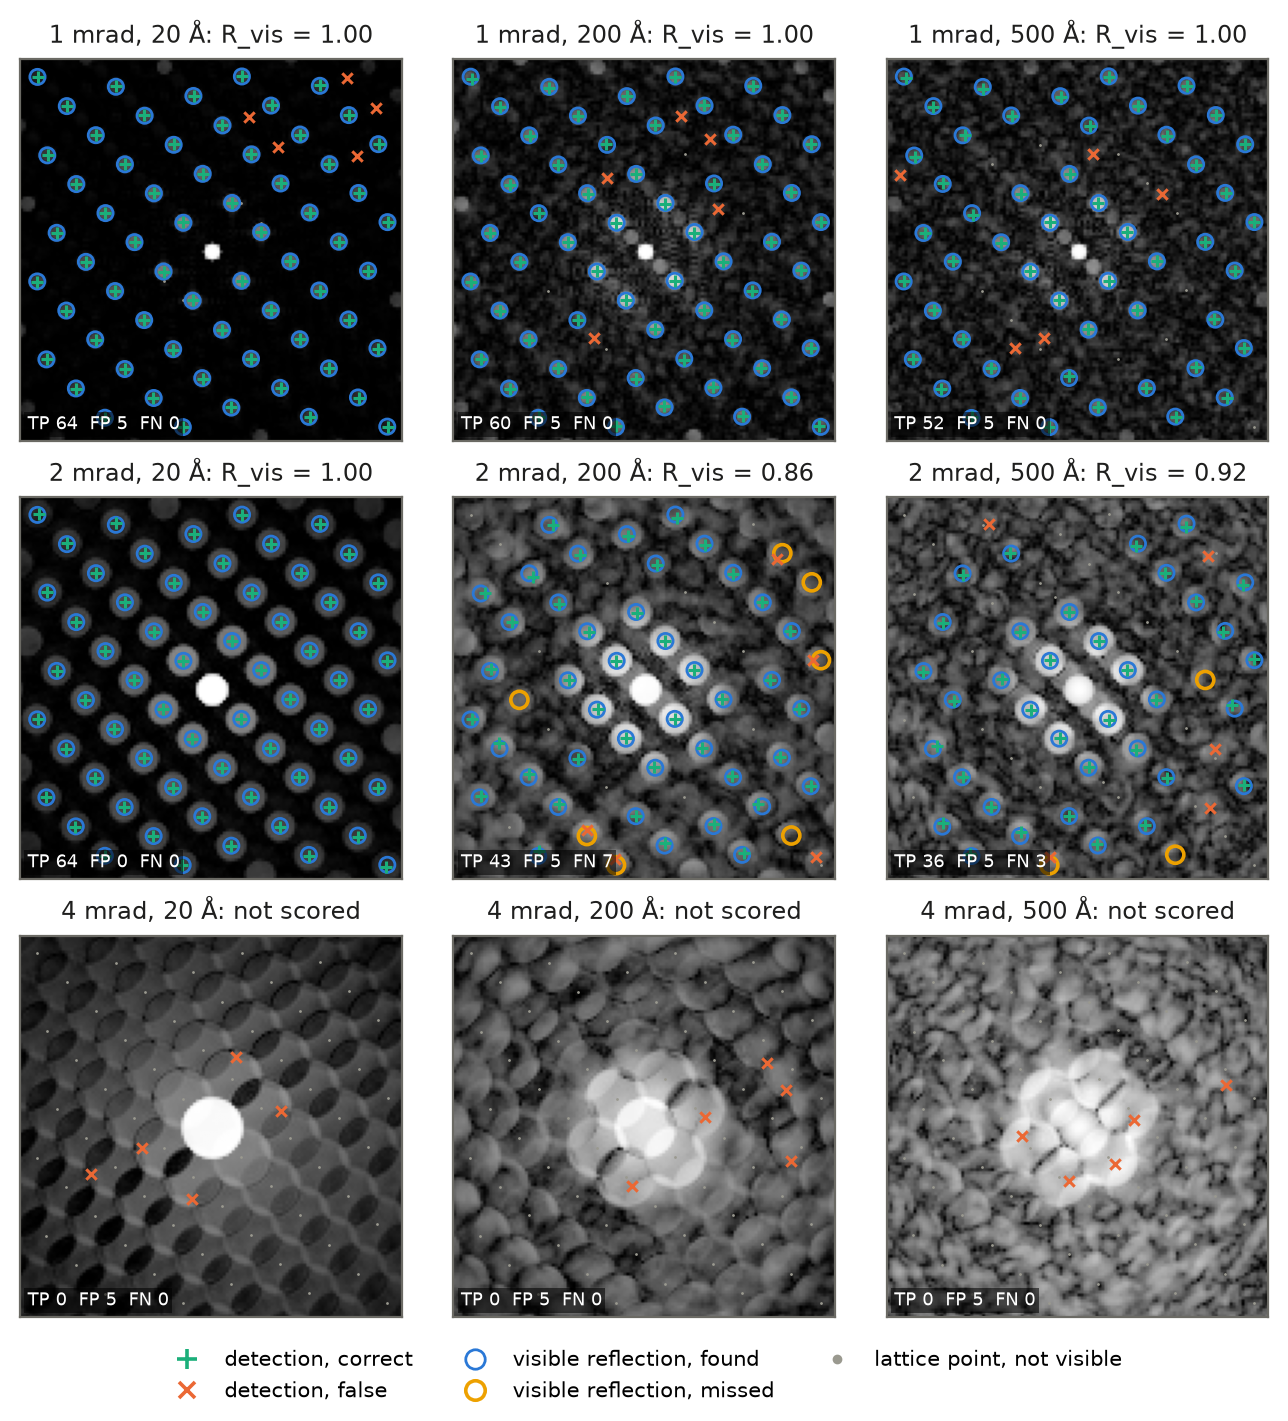
\includegraphics[width=\linewidth]{overlay_ZrSn3.png}
  \caption{ZrSn$_3$, layout and symbols as in \cref{fig:sio2} ($\eta = 0.38$, $0.68$, $1.43$). At \SI{4}{\milli\radian}
  the disks overlap everywhere, no reflection is visible, and the five false detections allowed per image fall on the
  direct beam and on overlap regions.}
  \label{fig:zrsn3}
\end{figure}

\subsection{Summary}
Overlap defeats the disk--ring filter through four effects, which set in at the same point, $\eta \approx 0.8$--$1$:
\begin{enumerate}
  \item the ring falls on neighbouring disks and their intensity is subtracted from the response at the true centre
        (\cref{eq:response}); this alone loses half of the disks in the synthetic test;
  \item interference makes overlapping disks non-uniform and sometimes darker than their surroundings, which the filter
        cannot detect;
  \item the visibility test fails for the same reason, so $\Rvis$ stays high while $\Rall$ collapses;
  \item the peaks that remain are shifted and broadened, and the localisation error grows five-fold.
\end{enumerate}
None of these is a defect of a parameter choice: they follow from looking for disks one at a time when the disks are no
longer separate.

%══════════════════════════════════════════════════════════════════════════════
\section{Practical guidance}\label{sec:guide}
\Cref{eq:ringcond} with $r = \kappa\alpha$ gives the largest probe semi-angle at which the ring still lies on background:
\begin{equation}
  \alpha_{\max} = \frac{s - g - w}{2\kappa} \approx \frac{s - \SI{3}{px}}{\SI{5}{px\per\milli\radian}} .
  \label{eq:alphamax}
\end{equation}
\Cref{tab:alphamax} lists $\alpha_{\max}$ for representative lattices. It agrees with the results: AlCo$_3$ and ZrSn$_3$
($\alpha_{\max} = \SI{2.2}{\milli\radian}$) work at 1 and \SI{2}{\milli\radian} and fail at \SI{4}{\milli\radian};
SiO$_2$ (\SI{1.1}{\milli\radian}) works at \SI{1}{\milli\radian} and already loses half of its lattice reflections at
\SI{2}{\milli\radian}. For dense lattices ($s < \SI{5}{px}$) no practical probe angle keeps the disks apart. When a larger
angle is required, the disks have to be found jointly rather than one at a time, for example by fitting overlapping disks
constrained to a lattice to the whole pattern.

\begin{table}[!htbp]
  \centering
  \caption{Largest probe semi-angle that keeps the filter ring on background, \cref{eq:alphamax}, with
  $\kappa = \SI{2.46}{px\per\milli\radian}$ (mean of $r/\alpha$ over the three angles).}
  \label{tab:alphamax}
  \small
  \begin{tabular}{l c c l}
    \toprule
    Crystal & $s$ (px) & $\alpha_{\max}$ (mrad) & Observed \\
    \midrule
    Ba$_2$Mn$_3$O$_8$  & 18.1 & 3.07 & good at 1 and 2 mrad \\
    AlCo$_3$, ZrSn$_3$ & 13.8--14.0 & 2.2 & good at 1 and 2 mrad, fails at 4 mrad \\
    SiO$_2$            & 8.6  & 1.14 & good at 1 mrad, $\Rall$ halved at 2 mrad \\
    HoTe$_3$           & 6.3  & 0.67 & $\Rvis = 0.36$ already at 1 mrad \\
    SiI$_3$            & 3.8  & 0.16 & $\eta = 1.4$ already at 1 mrad \\
    \bottomrule
  \end{tabular}
\end{table}

%══════════════════════════════════════════════════════════════════════════════
\section{Limitations}
\begin{itemize}
  \item The threshold of each image is chosen on that image, which is optimistic; a fair protocol fixes it on some images
        and applies it to others.
  \item The spacing $s$ counts every lattice point with at least \SI{5}{\percent} of the strongest $V$, including
        reflections that are weak in $M$. For some dense lattices $\eta$ therefore overstates the overlap between the bright
        disks (six crystals have $\eta \ge 1$ at \SI{1}{\milli\radian} but still $\Rvis \ge 0.8$).
  \item The visibility test shares the filter's disk--ring geometry, so part of the fall in visible reflections under
        overlap is a property of the definition; $\Rall$ does not have this problem.
  \item The patterns are simulated and noise-free. Detector data add Poisson noise, which would require a
        variance-stabilising transform before the logarithm.
\end{itemize}

\appendix
\section{Parameters and code}
\begin{table}[!htbp]
  \centering
  \caption{All parameters. Only $\varepsilon$ and $\rho$ were chosen from the data; $r$ follows from the probe.}
  \label{tab:params}
  \small
  \begin{tabular}{lll}
    \toprule
    Parameter & Value & Role \\
    \midrule
    $\varepsilon$   & $10^{-4}$ & true-log floor, \cref{eq:truelog} \\
    $r$             & 2.6 / 4.7 / 9.9 px & disk radius at 1 / 2 / 4 mrad, \cref{eq:probe} \\
    $g$, $w$        & 1 px, 2 px & gap and ring width, \cref{eq:sets} \\
    $\rho$          & 4 px & minimum distance between detected peaks \\
    Matching radius & 2 px & detection counted as correct \\
    Visibility      & disk $\ge 3\times$ ring, $\ge 10^{-3}$ of brightest & visible reflections \\
    Operating point & $\le 5$ false detections per image & threshold, chosen per image \\
    \bottomrule
  \end{tabular}
\end{table}

\paragraph{Code and data.}
\begin{itemize}
  \item Method: \path{notebooks/dummy_data_explore.ipynb}, functions \path{true_log01},\\
        \path{disc_ring_kernel}, \path{disc_centre_map} and \path{pick_peaks}.
  \item Per-image evaluation: \path{notebooks/scripts/run_per_image.py}; results in\\
        \path{notebooks/results/per_image_recall.csv}.
  \item Overlap analysis and synthetic experiment: \path{notebooks/scripts/run_overlap_analysis.py}; results in\\
        \path{notebooks/results/overlap_real.csv} and \path{overlap_synthetic.csv}.
  \item Figures: \path{notebooks/tutorial/make_figs.py}.
\end{itemize}

\end{document}
